\documentclass{standalone}
\usepackage{tikz}
\usetikzlibrary{patterns, positioning}

\begin{document}
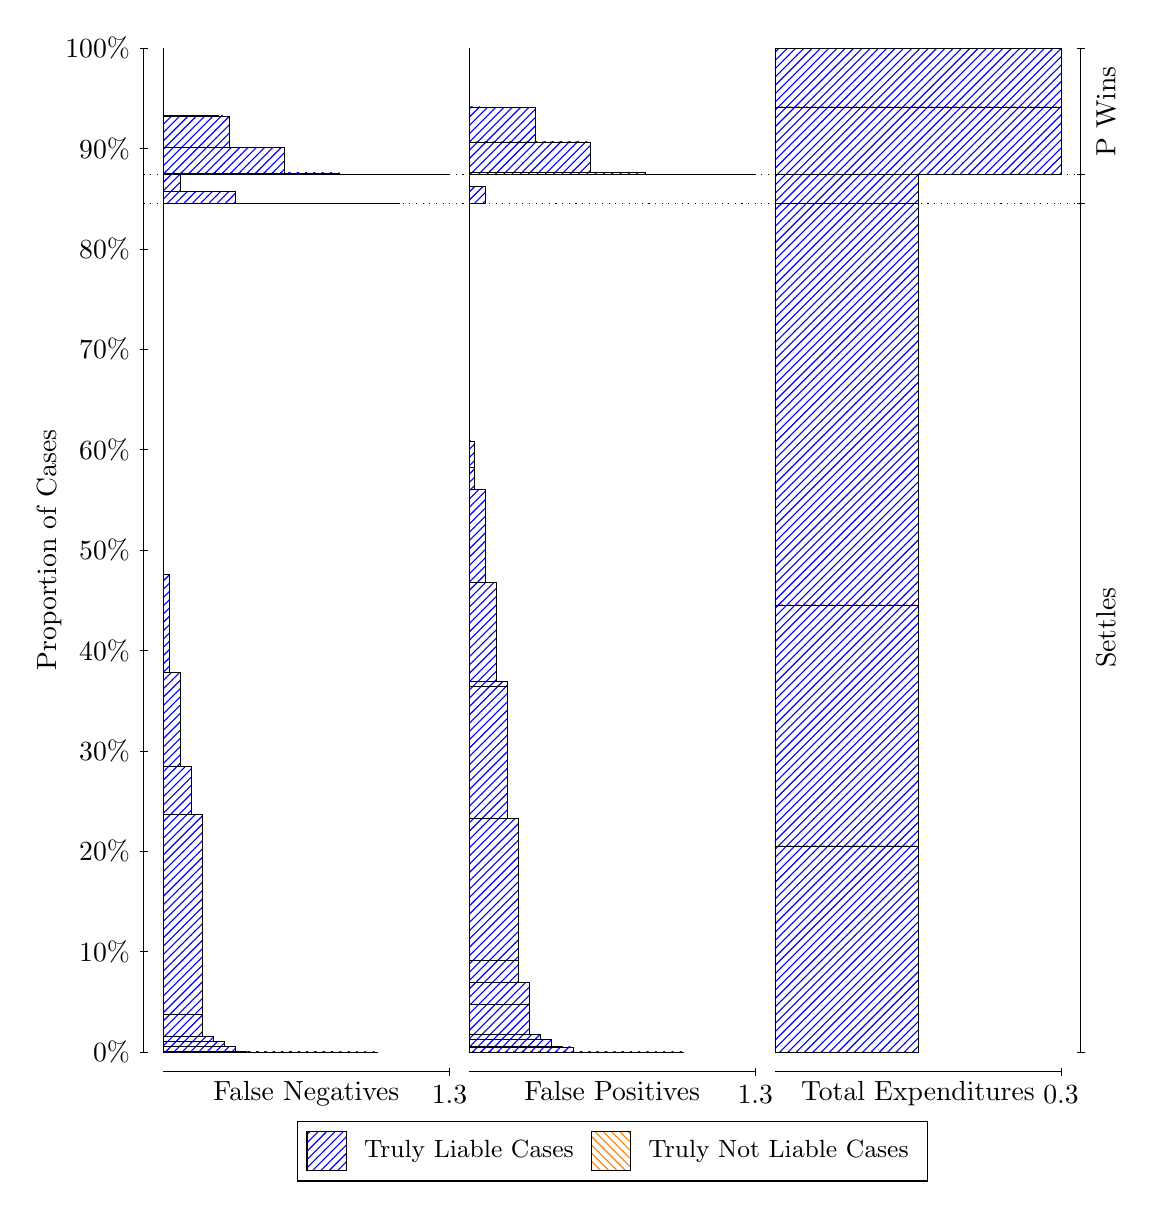
\begin{tikzpicture}
\draw[black, very thin] (1.5,1.75) -- (1.5,14.5);
\node[rotate=90, anchor=center] at (0.3, 8.125) {Proportion of Cases};
\draw[black, very thin] (1.45,1.75) -- (1.55,1.75);
\node[anchor=east] at (1.45, 1.75) {0\%};
\draw[black, very thin] (1.45,3.025) -- (1.55,3.025);
\node[anchor=east] at (1.45, 3.025) {10\%};
\draw[black, very thin] (1.45,4.3) -- (1.55,4.3);
\node[anchor=east] at (1.45, 4.3) {20\%};
\draw[black, very thin] (1.45,5.575) -- (1.55,5.575);
\node[anchor=east] at (1.45, 5.575) {30\%};
\draw[black, very thin] (1.45,6.85) -- (1.55,6.85);
\node[anchor=east] at (1.45, 6.85) {40\%};
\draw[black, very thin] (1.45,8.125) -- (1.55,8.125);
\node[anchor=east] at (1.45, 8.125) {50\%};
\draw[black, very thin] (1.45,9.4) -- (1.55,9.4);
\node[anchor=east] at (1.45, 9.4) {60\%};
\draw[black, very thin] (1.45,10.675) -- (1.55,10.675);
\node[anchor=east] at (1.45, 10.675) {70\%};
\draw[black, very thin] (1.45,11.95) -- (1.55,11.95);
\node[anchor=east] at (1.45, 11.95) {80\%};
\draw[black, very thin] (1.45,13.225) -- (1.55,13.225);
\node[anchor=east] at (1.45, 13.225) {90\%};
\draw[black, very thin] (1.45,14.5) -- (1.55,14.5);
\node[anchor=east] at (1.45, 14.5) {100\%};

\draw[black, very thin] (13.4,1.75) -- (13.4,14.5);
\draw[black, very thin] (13.35,1.75) -- (13.45,1.75);
\node[anchor=west] at (13.35, 1.75) {};
\draw[black, very thin] (13.35,12.526) -- (13.45,12.526);
\node[anchor=west] at (13.35, 12.526) {};
\draw[black, very thin] (13.35,12.891) -- (13.45,12.891);
\node[anchor=west] at (13.35, 12.891) {};
\draw[black, very thin] (13.35,14.5) -- (13.45,14.5);
\node[anchor=west] at (13.35, 14.5) {};

\draw[black, very thin, pattern color=blue, pattern=north east lines] (1.75,1.75) rectangle (4.475,1.75);
\draw[black, very thin, pattern color=blue, pattern=north east lines] (1.75,1.75) rectangle (4.1955,1.75);
\draw[black, very thin, pattern color=blue, pattern=north east lines] (1.75,1.75) rectangle (3.916,1.75);
\draw[black, very thin, pattern color=blue, pattern=north east lines] (1.75,1.75) rectangle (3.7763,1.75);
\draw[black, very thin, pattern color=blue, pattern=north east lines] (1.75,1.75) rectangle (3.6365,1.75);
\draw[black, very thin, pattern color=blue, pattern=north east lines] (1.75,1.75) rectangle (3.4968,1.75);
\draw[black, very thin, pattern color=blue, pattern=north east lines] (1.75,1.75) rectangle (3.3571,1.75);
\draw[black, very thin, pattern color=blue, pattern=north east lines] (1.75,1.75) rectangle (3.2173,1.75);
\draw[black, very thin, pattern color=blue, pattern=north east lines] (1.75,1.75) rectangle (3.0776,1.75);
\draw[black, very thin, pattern color=blue, pattern=north east lines] (1.75,1.75) rectangle (2.9378,1.7506);
\draw[black, very thin, pattern color=blue, pattern=north east lines] (1.75,1.7506) rectangle (2.7981,1.7552);
\draw[black, very thin, pattern color=blue, pattern=north east lines] (1.75,1.7552) rectangle (2.6583,1.8185);
\draw[black, very thin, pattern color=blue, pattern=north east lines] (1.75,1.8185) rectangle (2.5186,1.8837);
\draw[black, very thin, pattern color=blue, pattern=north east lines] (1.75,1.8837) rectangle (2.3788,1.9508);
\draw[black, very thin, pattern color=blue, pattern=north east lines] (1.75,1.9508) rectangle (2.2391,2.2247);
\draw[black, very thin, pattern color=blue, pattern=north east lines] (1.75,2.2247) rectangle (2.2391,4.7664);
\draw[black, very thin, pattern color=blue, pattern=north east lines] (1.75,4.7664) rectangle (2.0994,5.3779);
\draw[black, very thin, pattern color=blue, pattern=north east lines] (1.75,5.3779) rectangle (1.9596,6.567);
\draw[black, very thin, pattern color=blue, pattern=north east lines] (1.75,6.567) rectangle (1.8199,7.8178);
\draw[black, very thin, pattern color=orange, pattern=north west lines] (1.75,7.8178) rectangle (1.75,7.8178);
\draw[black, very thin, pattern color=blue, pattern=north east lines] (1.75,7.8178) rectangle (1.75,12.526);
\draw[black, very thin, pattern color=blue, pattern=north east lines] (1.75,12.526) rectangle (4.7545,12.526);
\draw[black, very thin, pattern color=blue, pattern=north east lines] (1.75,12.526) rectangle (4.0558,12.526);
\draw[black, very thin, pattern color=blue, pattern=north east lines] (1.75,12.526) rectangle (3.3571,12.526);
\draw[black, very thin, pattern color=blue, pattern=north east lines] (1.75,12.526) rectangle (2.6583,12.679);
\draw[black, very thin, pattern color=blue, pattern=north east lines] (1.75,12.679) rectangle (1.9596,12.891);
\draw[black, very thin, pattern color=orange, pattern=north west lines] (1.75,12.891) rectangle (1.75,12.891);
\draw[black, very thin, pattern color=blue, pattern=north east lines] (1.75,12.891) rectangle (5.3833,12.891);
\draw[black, very thin, pattern color=blue, pattern=north east lines] (1.75,12.891) rectangle (4.6846,12.891);
\draw[black, very thin, pattern color=blue, pattern=north east lines] (1.75,12.891) rectangle (3.9859,12.913);
\draw[black, very thin, pattern color=blue, pattern=north east lines] (1.75,12.913) rectangle (3.8462,12.913);
\draw[black, very thin, pattern color=blue, pattern=north east lines] (1.75,12.913) rectangle (3.2872,13.243);
\draw[black, very thin, pattern color=blue, pattern=north east lines] (1.75,13.243) rectangle (3.1474,13.243);
\draw[black, very thin, pattern color=blue, pattern=north east lines] (1.75,13.243) rectangle (2.5885,13.639);
\draw[black, very thin, pattern color=blue, pattern=north east lines] (1.75,13.639) rectangle (2.4487,13.642);
\draw[black, very thin, pattern color=blue, pattern=north east lines] (1.75,13.642) rectangle (1.8897,13.642);
\draw[black, very thin, pattern color=orange, pattern=north west lines] (1.75,13.642) rectangle (1.75,13.642);
\draw[black, very thin, pattern color=blue, pattern=north east lines] (1.75,13.642) rectangle (1.75,14.5);
\draw[black, very thin, pattern color=orange, pattern=north west lines] (5.6333,1.75) rectangle (8.3583,1.75);
\draw[black, very thin, pattern color=blue, pattern=north east lines] (5.6333,1.75) rectangle (8.3583,1.75);
\draw[black, very thin, pattern color=orange, pattern=north west lines] (5.6333,1.75) rectangle (7.7994,1.75);
\draw[black, very thin, pattern color=blue, pattern=north east lines] (5.6333,1.75) rectangle (7.7994,1.75);
\draw[black, very thin, pattern color=blue, pattern=north east lines] (5.6333,1.75) rectangle (7.6596,1.75);
\draw[black, very thin, pattern color=orange, pattern=north west lines] (5.6333,1.75) rectangle (7.5199,1.75);
\draw[black, very thin, pattern color=blue, pattern=north east lines] (5.6333,1.75) rectangle (7.5199,1.75);
\draw[black, very thin, pattern color=orange, pattern=north west lines] (5.6333,1.75) rectangle (7.2404,1.75);
\draw[black, very thin, pattern color=blue, pattern=north east lines] (5.6333,1.75) rectangle (7.2404,1.75);
\draw[black, very thin, pattern color=blue, pattern=north east lines] (5.6333,1.75) rectangle (7.1006,1.7506);
\draw[black, very thin, pattern color=orange, pattern=north west lines] (5.6333,1.7506) rectangle (6.9609,1.7506);
\draw[black, very thin, pattern color=blue, pattern=north east lines] (5.6333,1.7506) rectangle (6.9609,1.7513);
\draw[black, very thin, pattern color=blue, pattern=north east lines] (5.6333,1.7513) rectangle (6.9609,1.8155);
\draw[black, very thin, pattern color=blue, pattern=north east lines] (5.6333,1.8155) rectangle (6.8212,1.8179);
\draw[black, very thin, pattern color=orange, pattern=north west lines] (5.6333,1.8179) rectangle (6.6814,1.8179);
\draw[black, very thin, pattern color=blue, pattern=north east lines] (5.6333,1.8179) rectangle (6.6814,1.91);
\draw[black, very thin, pattern color=blue, pattern=north east lines] (5.6333,1.91) rectangle (6.5417,1.9738);
\draw[black, very thin, pattern color=orange, pattern=north west lines] (5.6333,1.9738) rectangle (6.4019,1.9738);
\draw[black, very thin, pattern color=blue, pattern=north east lines] (5.6333,1.9738) rectangle (6.4019,2.3593);
\draw[black, very thin, pattern color=blue, pattern=north east lines] (5.6333,2.3593) rectangle (6.4019,2.6355);
\draw[black, very thin, pattern color=blue, pattern=north east lines] (5.6333,2.6355) rectangle (6.2622,2.9101);
\draw[black, very thin, pattern color=blue, pattern=north east lines] (5.6333,2.9101) rectangle (6.2622,4.7143);
\draw[black, very thin, pattern color=orange, pattern=north west lines] (5.6333,4.7143) rectangle (6.1224,4.7143);
\draw[black, very thin, pattern color=blue, pattern=north east lines] (5.6333,4.7143) rectangle (6.1224,6.3946);
\draw[black, very thin, pattern color=blue, pattern=north east lines] (5.6333,6.3946) rectangle (6.1224,6.4582);
\draw[black, very thin, pattern color=blue, pattern=north east lines] (5.6333,6.4582) rectangle (5.9827,7.709);
\draw[black, very thin, pattern color=blue, pattern=north east lines] (5.6333,7.709) rectangle (5.8429,8.8981);
\draw[black, very thin, pattern color=blue, pattern=north east lines] (5.6333,8.8981) rectangle (5.7032,9.1717);
\draw[black, very thin, pattern color=blue, pattern=north east lines] (5.6333,9.1717) rectangle (5.7032,9.5096);
\draw[black, very thin, pattern color=blue, pattern=north east lines] (5.6333,9.5096) rectangle (5.6333,12.526);
\draw[black, very thin, pattern color=orange, pattern=north west lines] (5.6333,12.526) rectangle (5.8429,12.526);
\draw[black, very thin, pattern color=blue, pattern=north east lines] (5.6333,12.526) rectangle (5.8429,12.738);
\draw[black, very thin, pattern color=blue, pattern=north east lines] (5.6333,12.738) rectangle (5.6333,12.891);
\draw[black, very thin, pattern color=orange, pattern=north west lines] (5.6333,12.891) rectangle (9.2667,12.891);
\draw[black, very thin, pattern color=blue, pattern=north east lines] (5.6333,12.891) rectangle (9.2667,12.891);
\draw[black, very thin, pattern color=orange, pattern=north west lines] (5.6333,12.891) rectangle (8.5679,12.891);
\draw[black, very thin, pattern color=blue, pattern=north east lines] (5.6333,12.891) rectangle (8.5679,12.891);
\draw[black, very thin, pattern color=orange, pattern=north west lines] (5.6333,12.891) rectangle (7.8692,12.891);
\draw[black, very thin, pattern color=blue, pattern=north east lines] (5.6333,12.891) rectangle (7.8692,12.921);
\draw[black, very thin, pattern color=orange, pattern=north west lines] (5.6333,12.921) rectangle (7.1705,12.921);
\draw[black, very thin, pattern color=blue, pattern=north east lines] (5.6333,12.921) rectangle (7.1705,13.308);
\draw[black, very thin, pattern color=orange, pattern=north west lines] (5.6333,13.308) rectangle (7.0308,13.308);
\draw[black, very thin, pattern color=blue, pattern=north east lines] (5.6333,13.308) rectangle (7.0308,13.308);
\draw[black, very thin, pattern color=blue, pattern=north east lines] (5.6333,13.308) rectangle (6.4718,13.749);
\draw[black, very thin, pattern color=orange, pattern=north west lines] (5.6333,13.749) rectangle (6.3321,13.749);
\draw[black, very thin, pattern color=blue, pattern=north east lines] (5.6333,13.749) rectangle (6.3321,13.749);
\draw[black, very thin, pattern color=blue, pattern=north east lines] (5.6333,13.749) rectangle (5.7731,13.752);
\draw[black, very thin, pattern color=orange, pattern=north west lines] (5.6333,13.752) rectangle (5.6333,13.752);
\draw[black, very thin, pattern color=blue, pattern=north east lines] (5.6333,13.752) rectangle (5.6333,14.5);
\draw[black, very thin, pattern color=orange, pattern=north west lines] (9.5167,1.75) rectangle (11.333,1.75);
\draw[black, very thin, pattern color=blue, pattern=north east lines] (9.5167,1.75) rectangle (11.333,4.3676);
\draw[black, very thin, pattern color=orange, pattern=north west lines] (9.5167,4.3676) rectangle (11.333,4.3676);
\draw[black, very thin, pattern color=blue, pattern=north east lines] (9.5167,4.3676) rectangle (11.333,7.4283);
\draw[black, very thin, pattern color=orange, pattern=north west lines] (9.5167,7.4283) rectangle (11.333,7.4283);
\draw[black, very thin, pattern color=blue, pattern=north east lines] (9.5167,7.4283) rectangle (11.333,12.526);
\draw[black, very thin, pattern color=orange, pattern=north west lines] (9.5167,12.526) rectangle (11.333,12.526);
\draw[black, very thin, pattern color=blue, pattern=north east lines] (9.5167,12.526) rectangle (11.333,12.891);
\draw[black, very thin, pattern color=orange, pattern=north west lines] (9.5167,12.891) rectangle (13.15,12.891);
\draw[black, very thin, pattern color=blue, pattern=north east lines] (9.5167,12.891) rectangle (13.15,13.752);
\draw[black, very thin, pattern color=orange, pattern=north west lines] (9.5167,13.752) rectangle (13.15,13.752);
\draw[black, very thin, pattern color=blue, pattern=north east lines] (9.5167,13.752) rectangle (13.15,14.5);
\draw[black, dotted] (1.5,12.526) -- (13.4,12.526);
\draw[black, dotted] (1.5,12.891) -- (13.4,12.891);
\draw[black, very thin] (1.75,1.5) -- (5.3833,1.5);
\node[anchor=north] at (3.5667, 1.5) {False Negatives};
\draw[black, very thin] (5.3833,1.45) -- (5.3833,1.55);
\node[anchor=north] at (5.3833, 1.45) {1.3};

\draw[black, very thin] (5.6333,1.5) -- (9.2667,1.5);
\node[anchor=north] at (7.45, 1.5) {False Positives};
\draw[black, very thin] (9.2667,1.45) -- (9.2667,1.55);
\node[anchor=north] at (9.2667, 1.45) {1.3};

\draw[black, very thin] (9.5167,1.5) -- (13.15,1.5);
\node[anchor=north] at (11.333, 1.5) {Total Expenditures};
\draw[black, very thin] (13.15,1.45) -- (13.15,1.55);
\node[anchor=north] at (13.15, 1.45) {0.3};

\node[black, centered, rotate=90] at (13.72, 7.138) {Settles};

\node[black, centered, rotate=90] at (13.72, 13.695) {P Wins};

\draw (7.449999999999999,1.5) node[draw=none] (baseCoordinate) {};
\begin{scope}[align=center]
        \matrix[scale=0.5, draw=black, below=0.5cm of baseCoordinate, nodes={draw}, column sep=0.1cm]{
            \node[rectangle, draw, minimum width=0.5cm, minimum height=0.5cm, pattern=north east lines, pattern color=blue] {}; &
            \node[draw=none, font=\small] (B) {Truly Liable Cases}; &
            \node[rectangle, draw, minimum width=0.5cm, minimum height=0.5cm, pattern=north west lines, pattern color=orange] {}; &
            \node[draw=none, font=\small] (B) {Truly Not Liable Cases}; \\
            };
\end{scope}

\end{tikzpicture}
\end{document}